\chapter{Buffer Overflow}

È un meccanismo che cerca di alterare il normale funzionamento 
di un eseguibile, andando ad operare su aree del programma 
non previste dal programmatore.

\section{Organizzazione della memoria di \\un programma}

Quando un programma gira in memoria, ha 5 sezioni:
\begin{itemize}
    \item a regione testo è fissata, contiene il codice del
    programma ed è a sola lettura
    \item La regione dati contiene i dati inizializzati e non
    inizializzati. Le variabili statiche vengono
    memorizzate in questa regione
    \item La regione BSS contiene static/global variabili non
    inizializzate
    \item Lo Heap è usato per dynamic memory allocation
    \item Lo stack è usato anche per allocare dinamicamente
    le variabili locali usate nelle funzioni, per passare
    parametri alle funzioni e per restituire valori dalle
    stesse.
\end{itemize}

\begin{figure}[ht]
    \centering
    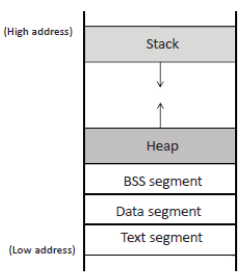
\includegraphics[width=0.55\linewidth]{chapters/images5/prog.png}
\end{figure}

\newpage
\section{Chiamate a funzioni}

\subsubsection{Un esempio}

\texttt{
    void func(int a, int b) \{ \\
     int x, y;\\
x = a + b;\\
y = a - b; \\ \}
}

\begin{figure}[ht]
    \centering
    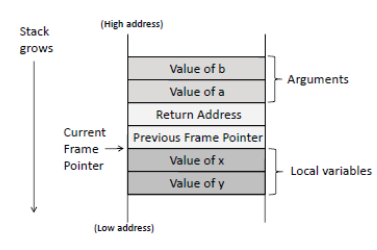
\includegraphics[width=0.75\linewidth]{chapters/images5/func.png}
\end{figure}

Il target dei buffer overflow è quello di sovrascrivere gli indirizzi di ritorno.


